\documentclass[conference]{IEEEtran}
\IEEEoverridecommandlockouts
% The preceding line is only needed to identify funding in the first footnote. If that is unneeded, please comment it out.
\usepackage{cite}
\usepackage{amsmath,amssymb,amsfonts}
\usepackage{algorithmic}
\usepackage{algorithm}
\usepackage{graphicx}
\usepackage{textcomp}
\usepackage{xcolor}
\usepackage{float}
\def\BibTeX{{\rm B\kern-.05em{\sc i\kern-.025em b}\kern-.08em
    T\kern-.1667em\lower.7ex\hbox{E}\kern-.125emX}}
\begin{document}

\renewcommand\IEEEkeywordsname{Keywords:}

\title{A Framework To Study Heuristic TSP Algorithms With Google Maps API}

\author{
\IEEEauthorblockN{Ajumal P A, Ananthakrishnan S, Anubhav Jain, Athreya H N, K Chandrasekaran}
\IEEEauthorblockA{\textit{Department of Computer Science \& Engineering}\\
\textit{National Institute of Technology Karnataka Surathkal} \\
Mangalore, India \\
}
}
\maketitle

\begin{abstract}
Millions of people depend on the navigation facilities available in smart-phones and web browsers for their daily commutes, planning long trips ahead of time, looking up places etc. Integration of GPS and compass made navigating anywhere in the world a trivial task. Today, there are several applications available that fit the purpose of navigation such as Waze, HereWeGo (previously known as Here Maps by Nokia), Google Maps, etc. When Google Maps was used to embark on a tour that will take us to chosen places by covering the least distance possible, it is observed that none of the aforementioned applications provide such a feature. In this paper, a framework is developed with Google Maps APIs to create such a feature. This problem is mapped to the Traveling salesman problem and tried to solve it using algorithms known for approximating TSP such as Artificial Bee Colony Algorithm, Particle Swarm Optimization and Two-opt Algorithm. The framework is tested with these algorithms and found that, Particle Swarm Optimization gives the best possible route.

\end{abstract}

\begin{IEEEkeywords}
Navigation, Google Maps, Tour, Traveling salesman problem, Artificial Bee Colony Algorithm, Particle Swarm Optimization and Two-opt Algorithm.
\end{IEEEkeywords}

\section{Introduction}
Google Maps is a popular application which lets a user navigate around places. In addition to the Android application, it is available as a web application. Google Maps for India has a two-wheeler mode that calculates the travel time in a different way. 

Google maps gives a very efficient way of routing the vehicle in real time with respect to distance as well as time. Usually, it collects the traffic data in real time and find routes with lesser traffic. It also gives real-time traffic data on the map which is very useful for the user to understand which route could be more congested(They use colors to show the traffic volume, red being the very congested route).
Initially, all the maps available online had only option to mark one source and destination, Later it improved by giving multiple destinations with one source, which really improved the user experience. They also incorporated multiple public means of transport like bus including timing and names of the buses.

With all these options, a lacking with planning capacity of the maps is felt. If the exact place name or location is known, user can point those and get the route from their current location and navigate in real-time. Yet the sequence of travel in order to complete the tour in minimum  amount of time is the information that is missing in this exercise. Doing this manually using maps is a tedious task as the user may have to permute through all the possible ways of going by marking on the map and the distance. It is cumbersome if the number of cities user wants to travel is very large.

A close look at this problem shows that every user wants to travel through a number of cities and come back to the same city. Intuitively, it's like a circle because the user will always want to come back to the place where he actually started. With a mapping of this problem to a graph with cities as nodes and path between them as edges, it can be formulated as a Hamiltonian cycle. In a Hamiltonian Cycle all the vertices in the graph must be visited without repetition. Mapping problems like this will give an idea of how to solve them because of the very high number of research has been already in this area.

Finding a Hamiltonian path with a number of cities can be mapped to a very famous problem of Travelling Salesman Problem. A brief description of the same will be followed in this section. A tremendous amount of work has been done with regard to TSP. It has become a de-facto benchmark for any new algorithm in the literature. Since TSP is a very old problem, there are near-perfect solutions to specific TSP problems with constraints, although the general TSP still remains unsolved. A popular program that was introduced in 1997 is the Concorde. It is developed by the University of Waterloo in ANSI C. Concorde is regarded as one of the best TSP solvers till date for symmetric TSP. Concorde is compared with other tools of its time here[1].

\subsection {Problem Statement}

The requirement is to choose multiple locations in the map and get a tour of those places covering the minimum possible distance or taking the least amount of time. Also, the tour should get us back to the starting point. To meet these requirements, testing of various map applications such as HereWeGo, Waze Maps and Google Maps was done. Among the applications that were tested, only Google Maps provided at least a feature to choose a maximum of 10 locations. The rest allows a user to choose only source and destination. Even then, the problem is Google Maps will give you a route according to the order you chose the locations. This route is not based on efficiency as opposed to the requirement. In this scenario, even if an efficient tour was available, this information would be, unfortunately, hidden from a Google Maps user. 

In this paper, a solution is proposed to this issue in the form of a web application. The Traveling Salesman Problem is based on the same grounds as this issue and a mapping can be done with this issue as an instance of the Traveling Salesman Problem. Now, the solution to this problem can be obtained by solving the Traveling Salesman Problem. Three popular algorithms are explored which are known for solving the Traveling Salesman Problem. A comparison study is done to find out which algorithm best suits the need in terms of providing the best tour.


\subsection {Travelling Salesman Problem}

Travelling Salesman problem is a very popular NP-Hard optimization problem. Traveling Salesman Problem can be stated as follows: Given N number of cities, a salesman needs to travel to all cities. In doing so, the salesman must be careful about two constraints. Firstly, he must visit a city exactly once and the other constraint is he must traverse through the N number of cities and return to his starting point by traveling the minimum distance possible. The solution to this problem is a list of cities in the order which allows for minimum distance traversal. Three algorithms are used to solve this problem so as to find a solution to the original problem. The algorithms are Artificial Bee Colony Algorithm, Particle Swarm Optimization, and Parallel Two-opt Algorithm. A brief description of these algorithms can be found below.
\linebreak
\par
The rest of the paper is organized as follows: In section 2, an explanation of algorithms used to solve TSP is done. A description of how the web application is implemented can be found in section 3. Then in the same section, comparisons of the performance of the said algorithms are made on the grounds of execution time and generation of the best route (Best route, in this case, is the route with the minimum distance or shortest time). Lastly, the paper ends with a conclusion.

\section {Related Works}
Some of the recent related work with regards to maps are cab-hailing apps. These apps use algorithms which exist to give the user the shortest-possible commute with reference to time and distance. Much of the other products based on maps focus on point-to-point routes based on the locations given by the user, in that order. Apps like Waze, provide real-time traffic information and road information so that the user gets the best information possible at the right time.

Vehicle routing problem is another specific version of the problem, which deals with customer pickup and delivery. Many algorithms have been developed to solve this problem[2][3][4].Researchers leveraged the problem of vehicle tracking and routing, guiding them in the right direction between two cities[5][6]. Another critical and important application is that the self-driving cars which are using maps to route themselves. This is such an important application that it is very difficult to imagine self-driving cars without maps data.

Tracking for safety purpose is another map related application which uses GPS to track the entire fleet of taxi service. This will allow the company/user to track its vehicles as well as improve the safety of passengers. There are two types of tracking: passive and active. When the GPS data is collected in a device but it is not transmitted, it is called passive tracking. Collected data is retrieved only when the vehicle returns to the company. This cannot ensure the safety of customers. In the case of active tracking, the data collected by various sensors are transmitted in near real-time. This ensures that the activities are supervised and safety of passengers is ensured.  

In the case of TSP, a large number of approximate algorithms have been developed.There are a number of real world problems which can  be generalized to TSP[7]. A broad area of research for TSP approximation is genetic algorithms. There are specific techniques to find the subsequent generations in GA and all of them are compared here[8]. Nature-inspired algorithms for solving TSP include Artificial Bee Colony Optimization[9], Ant Colony Optimization[10], Particle Swarm Optimization[11][12]. A hybrid method to solve TSP[13] is also in the literature which considers different algorithms for different situations. Since TSP can be broken down into sub-problems for some specific cases, these cases can be highly optimized with parallel coding architecture. Much work has been done with regards to solving TSP with parallel programs[14],[15]. All the above meta-heuristic algorithms have been adopted to take advantage of parallelization. A number of greedy algorithms are also developed as an approximation strategy to conquer TSP, like lin-kernighen, greedy 2-Opt, 2-mst, etc. 


\section{Algorithms}
\subsection {Artificial Bee Colony with SPV rule (ABC)}
Swarm-based meta-heuristic algorithm ABC is designed based on the behavior of honey bees. A Bee Colony has three kinds of bees: Employed bees, Onlooker bees, and Scout bees. Each of these bees serves a specific purpose. The number of solutions made for the initial permutation of the cities is called population size. The solutions are randomly initialized. The dimension of each solution will be of the number of cities. The fitness function will give you the cost of the solution which you pass from the population. 

ABC algorithm by itself cannot be used for solving the Traveling Salesman Problem. This is because ABC uses real number generation to obtain new solutions but Traveling Salesman Problem requires discrete values. This can be solved by applying SPV rule (Shortest Position Value)[16]. SPV rule will convert the random real numbers generated into discrete values in their increasing order. For eg. Consider an instance of TSP with 5 cities. Suppose ABC has generated  a solution [0.5, 2.5, 1.2, 4.5, 4.0]. SPV rule will convert this solution into [0, 2, 1, 4, 3]. Here, 4.5 is converted to 4 and 4.0 to 3 because the cities are named 0 to 4. The algorithm is as follows:


\begin{algorithm}[H]
\caption{Algorithm for ABC}
\begin{algorithmic}[1]
\STATE [Phase for Initialization]
\FOR {ps=0 to population size}
\FOR {nc=0 to no. of cities}
\STATE Randomly Initialize solutions
\STATE Use SPV rule to convert real sequence vector to discrete sequence vector
\ENDFOR 
\STATE Compute the fitness of the solution
\ENDFOR 

\REPEAT
\STATE [Phase for Employed Bees]

\FOR {eb=0 to no. of employed bees}
\FOR {nc=0 to no. of cities}
\STATE generate a new solution from existing solution
\STATE convert this solution to a discrete solution using SPV rule
\ENDFOR 


\STATE Calculate fitness of each individual
\IF {fitness of new solution is greater than existing solution}
\STATE solution = new solution
\ENDIF
\ENDFOR
\STATE Compute the probability of each individual
\STATE [Phase for Onlooker Bees]
\FOR {nb=0 to no. of onlooker bees}
\STATE select solution based on probability
\FOR {nc=0 to no. of cities}
\STATE generate a new solution
\STATE convert this solution to a discrete solution using SPV rule
\ENDFOR
\STATE Calculate fitness of each individual
\IF {fitness of new candidate greater than existing solution}
\STATE solution = new candidate solution
\ENDIF
\ENDFOR
\STATE [Phase for Scout Bees]
\IF {food sources are exhausted}
\STATE convert the employed bee to scout bee and search for solutions randomly
\ENDIF

\UNTIL {termination criteria is satisfied}
\end{algorithmic}
\end{algorithm}



\begin{table}[h!]
 \label{tab:table1}\caption{Experimental results for ABC}
  \begin{center}
    \begin{tabular}{l|c|r}
      \textbf{Number of Cities} & \textbf{Running Time (ms)} & \textbf{Path Cost (km)}\\
      \hline
      5 & 19 & 538\\
      10 & 36& ,4321\\
      15 & 59  & 7663\\
      20 & 96  & 10789\\ 
      25 & 133 & 15089\\
      30 & 173  & 18133\\
    \end{tabular}
  \end{center}
\end{table}


\subsection {Particle Swarm Optimization (PSO)}
In PSO, each candidate solution is called a particle and candidate solution is incrementally improved based on a desired property. Each particle moves across the solution space and  updates its velocity at regular interval of time to get the best position (personal best) and the globally best position is found out by the complete swarm (global best). To arrive at the best position, each particle utilize the present best solution known to them and global best solution which is available till now. PSO starts with a random group of solutions and then search is conducted incrementally. Particle swarm optimization to solve the traveling salesman problem uses the concept of swap operator and swap sequence and modifies operator if required[17]. 

\begin{algorithm}[H]
\caption{Algorithm for PSO}
\begin{algorithmic}[1]
\STATE Initialize Population
\REPEAT
\FOR{each particle P with position Xi}
\IF{Xi  is better than Pbest}
\STATE Pbest = Xi
\ENDIF
\ENDFOR 
\STATE Define Gbest , best position found so far by any neighbours of P
\FOR{each particle X}
\STATE Xv=Compute velocity(X, Pbest, Gbest)
\STATE Xp=Update position(Xp,Xv)
\ENDFOR
\UNTIL {termination criteria is satisfied} 
\end{algorithmic}
\end{algorithm} 



\begin{table}[h!]
  \begin{center}
    \label{tab:table2} \caption{Experimental results for PSO}
    \begin{tabular}{l|c|r}
      \textbf{Number of Cities} & \textbf{Running Time (ms)} & \textbf{Path Cost (km)}\\
      \hline
      5 & 32 & 538\\
      10 & 39 & 3990\\
      15 & 46 & 6946\\
      20 & 59 & 9936\\ 
      25 & 73 & 14669\\
      30 & 82 & 17767\\
    \end{tabular}
  \end{center}
\end{table}




\subsection {Parallel Two-opt Algorithm (PTO)}
2-Opt is a local search algorithm for solving TSP. The main idea with 2-Opt is that it takes 2 edges that are crossing over each other and straightens them out so that the distance travelled will be lesser.



\newlength\myindent
\setlength\myindent{2em}
\newcommand\bindent{%
  \begingroup
  \setlength{\itemindent}{\myindent}
  \addtolength{\algorithmicindent}{\myindent}
}
\newcommand\eindent{\endgroup}
\begin{algorithm}[H]
\caption{Algorithm for PTO}
\begin{algorithmic}[1]
\STATE 2-Opt (route, i, j)
\bindent
\STATE copy route from 0 to i-1 to new-route
\STATE copy route from i to j in reverse order to new route
\STATE copy route from j to end to new-route
\STATE return new-route
\eindent
\REPEAT
\STATE cur-distance = calculateDistance(currentRoute)
\FOR {i from 1 to number-of-nodes}
\FOR {k from i+1 to number-of-nodes} 
\STATE new-route = 2-Opt(existing-route, i, k)
\STATE new-dist = calculateDistance(new-route)
\IF {new-dist \textless cur-dist}
\STATE existing-route = new-route
\ENDIF
\ENDFOR
\ENDFOR 
\UNTIL {no improvements are found}
\end{algorithmic}
\end{algorithm} 




\begin{table}[h!]
  \begin{center}
    \label{tab:table3} \caption{Experimental results for PTO}
    \begin{tabular}{l|c|r}
      \textbf{Number of Cities} & \textbf{Running Time (ms)} & \textbf{Path Cost (km)}\\
      \hline
      5 & 574 & 545\\
      10 & 580 & 5310\\
      15 & 555 & 10221\\
      20 & 598 & 13599\\ 
      25 & 587 & 16713\\
      30 & 583 & 19169\\
    \end{tabular}
  \end{center}
\end{table}



Here, a parallel implementation of the 2-Opt algorithm is used. CUDA is a framework developed by NVIDIA for their graphics cards. CUDA lets you write serial “kernels” which are parallelized by the compiler with GCC at its back-end. NVCC is the compiler which converts the program into parallel code. When the program is run, it is first copied into the GPU memory and then executed. This causes an overhead for any program that is executed on the GPU. 

 The algorithm here utilizes the parallel processing capabilities of Tesla K40 GPU and is able to outperform the other algorithms when the number of cities is very large.If smaller values of n(number of cities) are considered for TSP, the program is actually slower than the serial code, but as the n value increases, the overhead becomes less significant and reaches to a point where the parallel code is orders of magnitude higher than serial code. The architecture of the code is in such a way that the cost-matrix is copied onto the device from CPU and the code which identifies the 2-Opt routes and corrects them in the graph is run simultaneously on hundreds of streaming multiprocessors[18]. 

 Considering the use case scenarios of the web application intended to work, this algorithm is unable to leverage it’s parallel processing capabilities because the algorithm takes significant overhead to load the program into GPU memory, hence for a fewer number of cities it is not suitable.

\begin{table}[h!]
  \begin{center}
    \label{tab:table4} \caption{Experimental results for Google Maps Application}
    \begin{tabular}{l|c|r}
      \textbf{Number of Cities} & \textbf{Path Cost (km)}\\
      \hline
      5 & 693\\
      10 & 5771\\
      15 & 9163\\
      20 & 13839\\ 
      25 & 17689\\
      30 & 21333\\
    \end{tabular}
    
  \end{center}
\end{table}


\section {Implementation}

For implementation purpose, Google maps API is used. For rendering and locating a node (marker), ‘map’ and ‘geocoder’ service provided by Google are used. Google Maps API also gives the information about the latitude, longitude and place address. For fetching the road distance between all the pairs of the cities, distance matrix service provided by Google is used. It takes latitude and longitude as input and returns road distance and time required to cover that distance.

Input data (complete graph) is created which contains distance information of every pair of nodes. After this, back-end is called using web service and give this complete graph for further processing.

A web server is used to receive the input from front-end, This complete graph is then converted into an adjacency matrix. The algorithms (PSO or ABC or PTO) is executed in the back-end which takes this adjacency matrix as input and gives us minimum cost route. The output will be sent to the front-end.

Directions API of Google is used to render the output on the map, which renders the “driving” mode route between the cities.

All executions were repeated 10 times using major cities within India. Cities are selected in the range starting from 5 and a maximum of 30 cities. As the tests were run, two metrics were measured: (i) running time and (ii) the cost of the tour generated by each algorithm. The results are shown in Fig1 and Fig2. It is evident from the results that all the algorithms that were employed give a far better solution than that of Google Maps. It is also found that PSO is giving the best cost solution among all the algorithms after 10 cities.

\begin{figure}[htbp]
\centerline{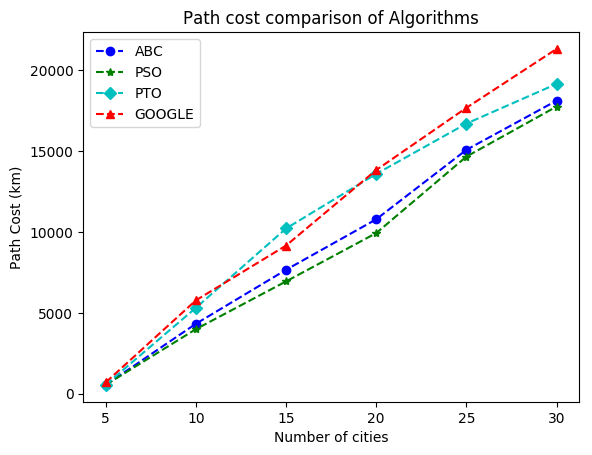
\includegraphics[width=\columnwidth]{pathcost.png}}
\caption{Path cost comparison.}
\label{fig1}
\end{figure}

\begin{figure}[htbp]
\centerline{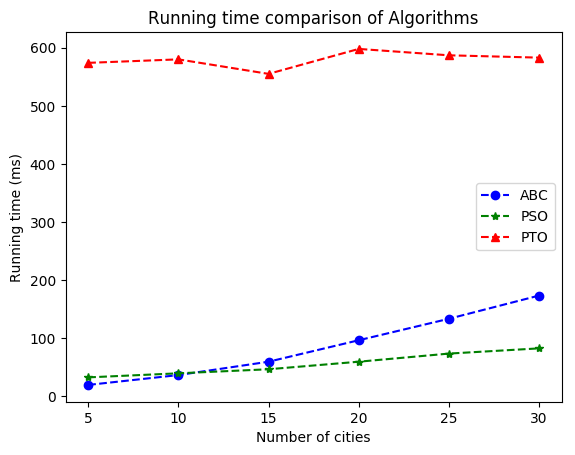
\includegraphics[width=\columnwidth]{runtime.png}}
\caption{Running time comparison.}
\label{fig2}
\end{figure}

The web application provides the user the ability to calculate the route based on distance or time. Two buttons are provided in the interface to serve this purpose. After marking all the desired locations, the user can click on either of the two buttons and the route with the desired property will be shown on the map. It is not the case that the route with minimum distance and the route with minimum time will be the same. There are cases in which the two routes are different. An example that illustrates this difference is shown on Figure 5 and Figure 6.

\section {Results}

Figure 1 shows the path cost comparison of algorithms that were implemented. The data was collected for routes with minimum distance. The tests were started with 5 cities and gradually went up to 30 cities. PSO algorithm gives the best performance when only 10 cities are selected. The Artificial Bee Colony algorithm gives almost the same performance as PSO.  This trend is continued throughout the test. Meanwhile, Google’s algorithm gives the worst performance overall. It performs slightly worse than PTO when tested on 10 cities. At 15 cities, Google’s algorithm better performed than PTO. As the number of cities was increased further, the performance of Google’s algorithm kept on getting worse. This can be seen from the graph as for 30 cities, the cost of the route provided by Google’s algorithm is 21,333 km and PTO was able to give a cost of 19,169km. In each case, the PSO algorithm was able to perform consistently and gives the best cost among all the algorithms. The performance analysis of routes with minimum time is the same. This is because the algorithms cannot identify whether the input data given to it is time or distance based.

Figure 2 shows the running time comparison of the algorithms. Here, it can be see that the PSO algorithm gives almost consistent running time for the number of cities that were tested. In the case of ABC, the increase in number of cities from 15 took a toll on the running time. The PTO algorithm gave the worst running time of all averaging at 570 ms. 

Figures 3 and 4 compare the results shown by the web application with the results of Google Maps. 

Figures 5 and 6 show that the web application can be configured to provide optimal results either by distance or by time. Figure 5 shows the configuration where the most optimal route follows the minimal distance than other routes, whereas most optimal route in Figure 6 follows minimum time taken among all routes.


\begin{figure}[htbp]
\centerline{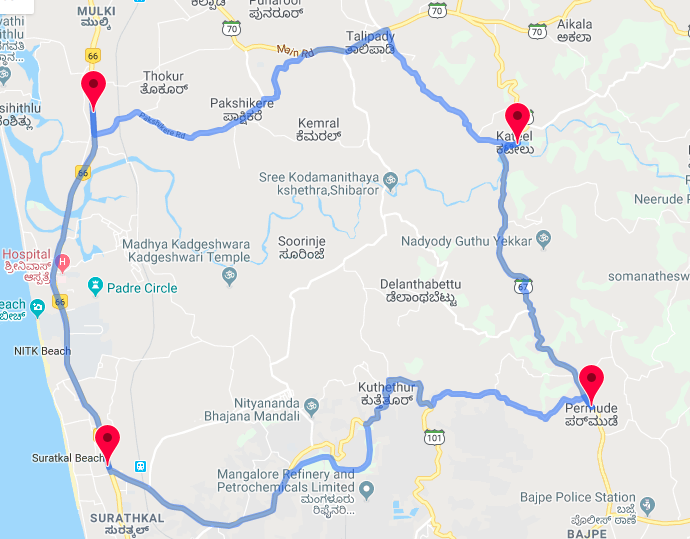
\includegraphics[width=\columnwidth]{tspResultApp.png}}
\caption{Tour planned by The Application(cost=37KM).}
\label{fig3}
\end{figure}


\begin{figure}[htbp]
\centerline{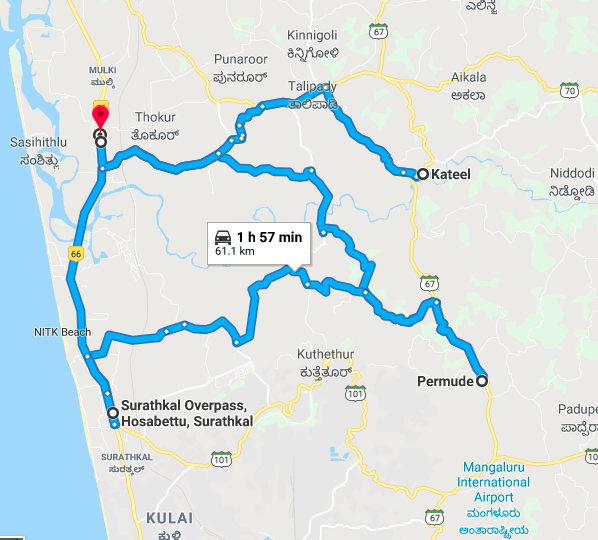
\includegraphics[width=\columnwidth]{tspResultGoogle.png}}
\caption{Tour planned by the Google Map (cost=61KM).}
\label{fig4}
\end{figure}


\begin{figure}[htbp]
\centerline{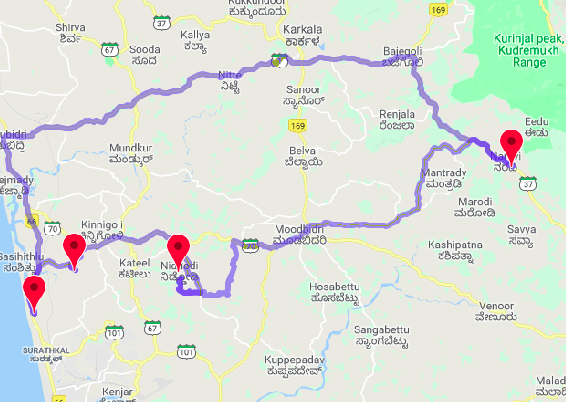
\includegraphics[width=\columnwidth]{distance.png}}
\caption{Route By Time.}
\label{fig5}
\end{figure}

\begin{figure}[htbp]
\centerline{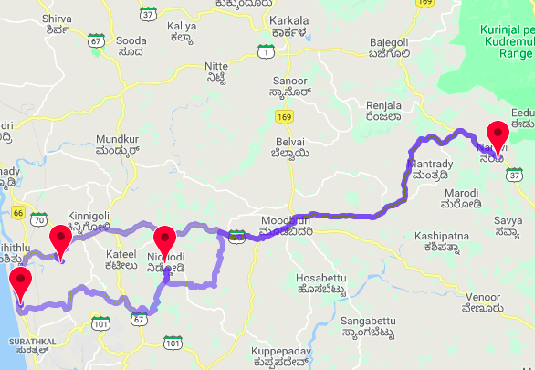
\includegraphics[width=\columnwidth]{time.png}}
\caption{Route By Distance.}
\label{fig6}
\end{figure}

\section {Conclusion \& Future Work}
A web application was created that provides an interface to select multiple locations. The application will give an optimal route back to the user. Depending on the choice, this route will be optimized either for minimum distance or minimum time. After comparing the three algorithms, the conclusion was made that (i) If the use case is limited to less than 10 cities, both ABC and PSO gives the same minimum cost, but PSO takes more time. So, ABC is recommended in this case. (ii) If the use case exceeds 10 cities, the running time as well as the quality of the route given by Particle Swarm Optimization is better than Artificial Bee Colony and 2-Opt. If number of cities chosen is more than 40, then 2-Opt outperforms other two algorithms, because it runs on GPU. Since it is required to load complete graph on GPU memory from CPU memory, it takes some time, i.e. it is not convenient to use 2-Opt for number of cities less 40. Hence, PSO is preferred in this case. In this paper, three algorithms are compared which are popular among the ones solving the Traveling Salesman Problem. As a continuation of this work, other algorithms can be explored and the framework can be improved to make it more generalized.


\begin{thebibliography}{00}

\bibitem{b1} C. Hitte, T. D. Lorentzen, R. Guyon, L. Kim, E. Cadieu, H. G. Parker, P. Quignon, J. K. Lowe, B. Gelfenbeyn, C. Andre, E. A. Ostrander and F. Galibert, "Comparison of MultiMap and TSP/CONCORDE for Constructing Radiation Hybrid Maps"  Journal of Heredity, Volume 94, Issue 1, 1 January 2003, pp. 9–13.

\bibitem{b2} E. Messaoud and A. E. Alaoui, "Hybrid ant colony system algorithm for the vehicle routing problem with dynamic customers and traffic factors," 2017 Intelligent Systems and Computer Vision (ISCV), Fez, 2017, pp. 1-4.

\bibitem{b3} S. Mingprasert and R. Masuchun, "Adaptive artificial bee colony algorithm for solving the capacitated vehicle routing problem," 2017 9th International Conference on Knowledge and Smart Technology (KST), Chonburi, 2017, pp. 23-27.

\bibitem{b4} L. Meng, C. Lin, H. Huang and X. Cai, "Vehicle routing plan based on ant colony and insert heuristic algorithm," 2016 35th Chinese Control Conference (CCC), Chengdu, 2016, pp. 2658-2662.

\bibitem{b5} A. Annouch, A. Bellabdaoui and J. Minkhar, "Split delivery and pickup vehicle routing problem with two-dimensional loading constraints," 2016 11th International Conference on Intelligent Systems: Theories and Applications (SITA), Mohammedia, 2016, pp. 1-6.

\bibitem{b6} Rui Li, Chun Cheng, Mingyao Qi and Weiwei Lai, "Design of dynamic vehicle routing system based on online map service," 2016 13th International Conference on Service Systems and Service Management (ICSSSM), Kunming, 2016, pp. 1-5.

\bibitem{b7} K. Ilavarasi and K. S. Joseph, "Variants of travelling salesman problem: A survey," International Conference on Information Communication and Embedded Systems (ICICES2014), Chennai, 2014, pp. 1-7.

\bibitem{b8} Noraini Mohd Razali and John Geraghty, "Genetic Algorithm Performance with Different Selection Strategies in Solving TSP", Proceedings of the World Congress on Engineering 2011 Vol II WCE 2011, Volume II, July 6 - 8, 2011, London, U.K.

\bibitem{b9} D. Karaboga and B. Gorkemli, "A combinatorial Artificial Bee Colony algorithm for traveling salesman problem," 2011 International Symposium on Innovations in Intelligent Systems and Applications, Istanbul, 2011, pp. 50-53.

\bibitem{b10} M. Dorigo and G. Di Caro, "Ant colony optimization: a new meta-heuristic," Proceedings of the 1999 Congress on Evolutionary Computation-CEC99 (Cat. No. 99TH8406), Washington, DC, USA, 1999, pp. 1470-1477 Vol. 2.

\bibitem{b11} Elizabeth F. G. Goldbarg, Marco C. Goldbarg and Givanaldo R. de Souza," Particle Swarm Optimization Algorithm for the Traveling Salesman Problem", Traveling Salesman Problem, Federico Greco (Ed.), pp. 202.

\bibitem{b12}  X.H.Shi, Y.C.Liang, H.P.Lee, C.Lu and Q.X.Wanga, "Particle swarm optimization-based algorithms for TSP and generalized TSP", Information Processing Letters 103, 2007, pp. 169–176.

\bibitem{b13} Mostafa Mahi, Omer Kaan Baykan and Halife Kodaz, "A new hybrid method based on Particle Swarm Optimization, Ant Colony Optimization and 3-Opt algorithms for Traveling Salesman Problem", Applied Soft Computing 30, 2015, pp. 484–490.

\bibitem{b14} U. Cekmez, M. Ozsiginan, and O. K. Sahingoz, "Adapting the GA approach to solve Traveling Salesman Problems on CUDA architecture," 2013 IEEE 14th International Symposium on Computational Intelligence and Informatics (CINTI), Budapest, 2013, pp. 423-428.

\bibitem{b15} R. Saxena, M. Jain, S. Bhadri and S. Khemka, "Parallelizing GA based heuristic approach for TSP over CUDA and OPENMP," 2017 International Conference on Advances in Computing, Communications and Informatics (ICACCI), Udupi, 2017, pp. 1934-1940.

\bibitem{b16} Nishant Pathak, Sudhanshu Prakash Tiwari, "Travelling Salesman Problem Using Bee Colony With SPV", International Journal of Soft Computing and Engineering (IJSCE), Volume-2, Issue-3, July 2012, pp.  2231-2307.

\bibitem{b17} Sarman K. Hadia, Arjun H. Joshi, Chaitalee K. Patel and Yogesh P Kosta, "Solving City Routing Issue with Particle Swarm Optimization", International Journal of Computer Applications (0975 – 888) Volume 47– No.15, June 2012, pp. 27-30.

\bibitem{b18} Kamil Rocki, Reiji Suda, "High Performance GPU Accelerated Local Optimization in TSP", IEEE 27th International Symposium on Parallel and Distributed Processing Workshops and PhD Forum, 2013, pp. 1788-1796.



\end{thebibliography}
\end{document}

 
